\subsection{\label{subsecMC}Comparison to Monte Carlo models}

%The measured multiplicity dependence of identified particle spectra in \pp\ collisions can 
%be readily compared to a variety of event generators employing significantly different physical 
%hypotheses. 

\begin{figure*}[t!]
  \begin{flushleft}
    \center{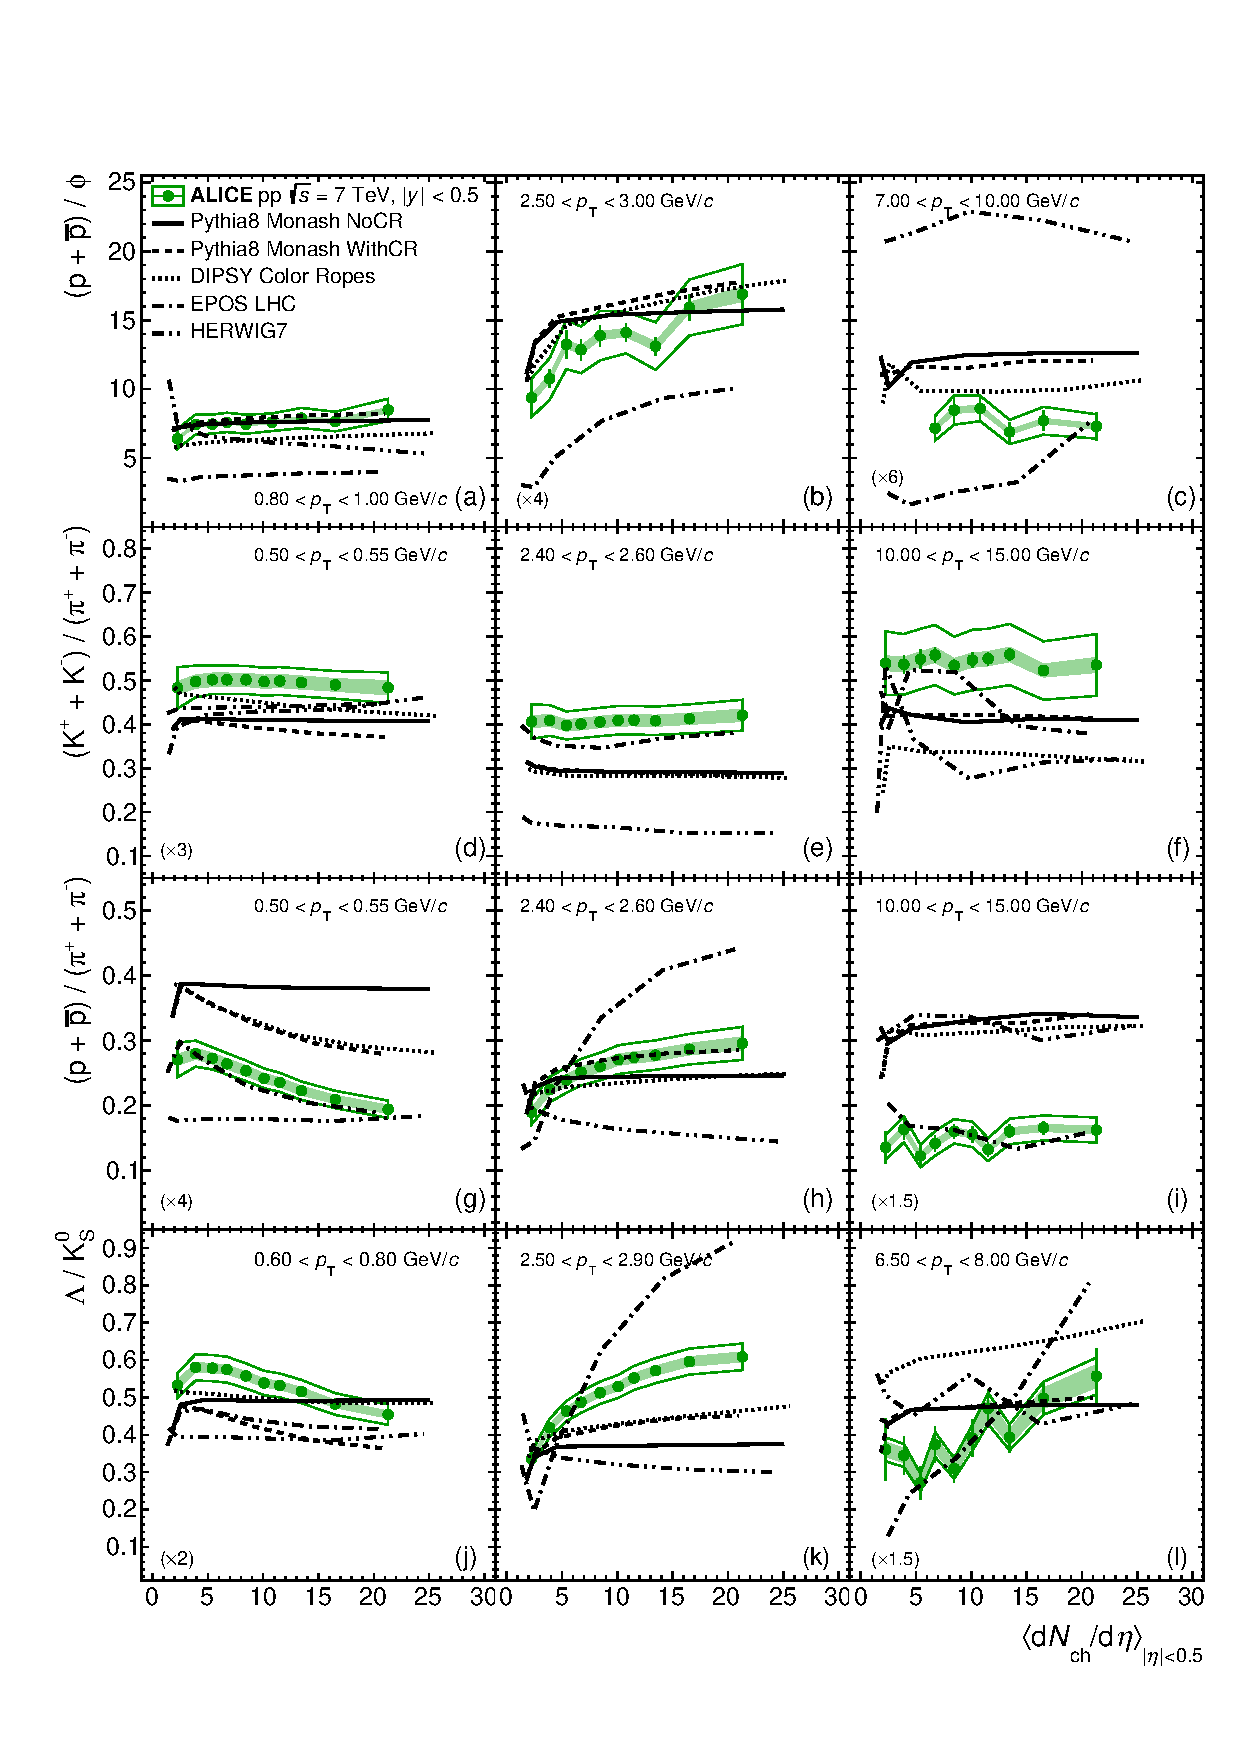
\includegraphics[width=\textwidth]{figures/Results_SpectraRatioVsMult_pp_MC_withProtonOverPhi.pdf}}
    \end{flushleft}
    \caption{Transverse momentum dependence of (a, b, c) \p/$\phi$~=~(p + \pbar)/$\phi$, (d, e, f) \kpi~=~(\kap + \kam)/(\pip + \pim),  (g, h, i) \ppi~=~(p + \pbar)/(\pip +
\pim) and (j, k, l) \lmb/\kzero\ yield ratios in (a, d, g, j) low-, (b, e, h, k) mid- and (c, f, i, l) high-\pt\ intervals compared to several Monte Carlo event generators. 
    Statistical uncertainties are shown as error bars, total systematic uncertainties are shown as hollow bands and multiplicity-uncorrelated 
    systematic uncertainties are shown as shaded bands.}
    \label{fig:RatiosVsPtVsMC}
\end{figure*}  


The multiplicity dependence of the \pt-differential \KTopi, \pTopi\ and \LtoKzero\ ratios 
 is compared to several Monte Carlo (MC) event generators, see Fig.~\ref{fig:RatiosVsPtVsMC}. 
 All predictions are obtained by performing selections on charged-particle 
 multiplicities in the V0M acceptance and are compared to data parametrically as a function of \avdNdeta, 
 as discussed in section \ref{subsecEventSelection}. 
 The PYTHIA8 
event generator in its Monash tune~\cite{Sjostrand:2007gs, Skands:2014pea} is only successful in describing the 
qualitative features of the evolution of the
baryon-to-meson ratios if color reconnection (CR) is allowed to occur, as observed already in previous 
work~\cite{PhysRevLett.111.042001}. 
In contrast to the string-model based PYTHIA, the HERWIG code implements hadronization in a clustering approach~\cite{Bahr:2008pv}. As shown in Fig.~\ref{fig:RatiosVsPtVsMC}, the abilities of HERWIG7 to describe particle production at low and intermediate \pt\ are still limited, but are currently being improved~\cite{Gieseke:2016fpz}.
DIPSY, a model in which fragmenting strings are allowed to form 
color ropes which then hadronize with a higher effective string tension~\cite{Bierlich:2014xba}, is also able to 
reproduce the decreasing (increasing) trend of the baryon-to-meson ratios at low (high) \pt, but fails in
describing the absolute values of these ratios. Furthermore, the EPOS-LHC event 
generator, which relies on parton-based Gribov-Regge theory and includes 
elements from hydrodynamics~\cite{Pierog:2013ria}, predicts increased baryon-to-meson ratios at intermediate
\pt\ as a consequence of radial flow, but overestimates the multiplicity dependence of these ratios and thus
fails to quantitatively reproduce the measurements reported here. 
Finally, essentially all models are able to reproduce the fact that the \KTopi\ ratio is multiplicity-independent, 
while not necessarily describing the absolute value well. These findings suggest that there is more than one 
physical mechanism that would lead to the dynamics
observed in \pt-differential identified particle ratios, and a systematic study of other observables
such as the flow coefficients $v_{n}$ is required in order to discriminate among the various possibilities. 

\begin{figure*}[t!]
  \begin{flushleft}
    \center{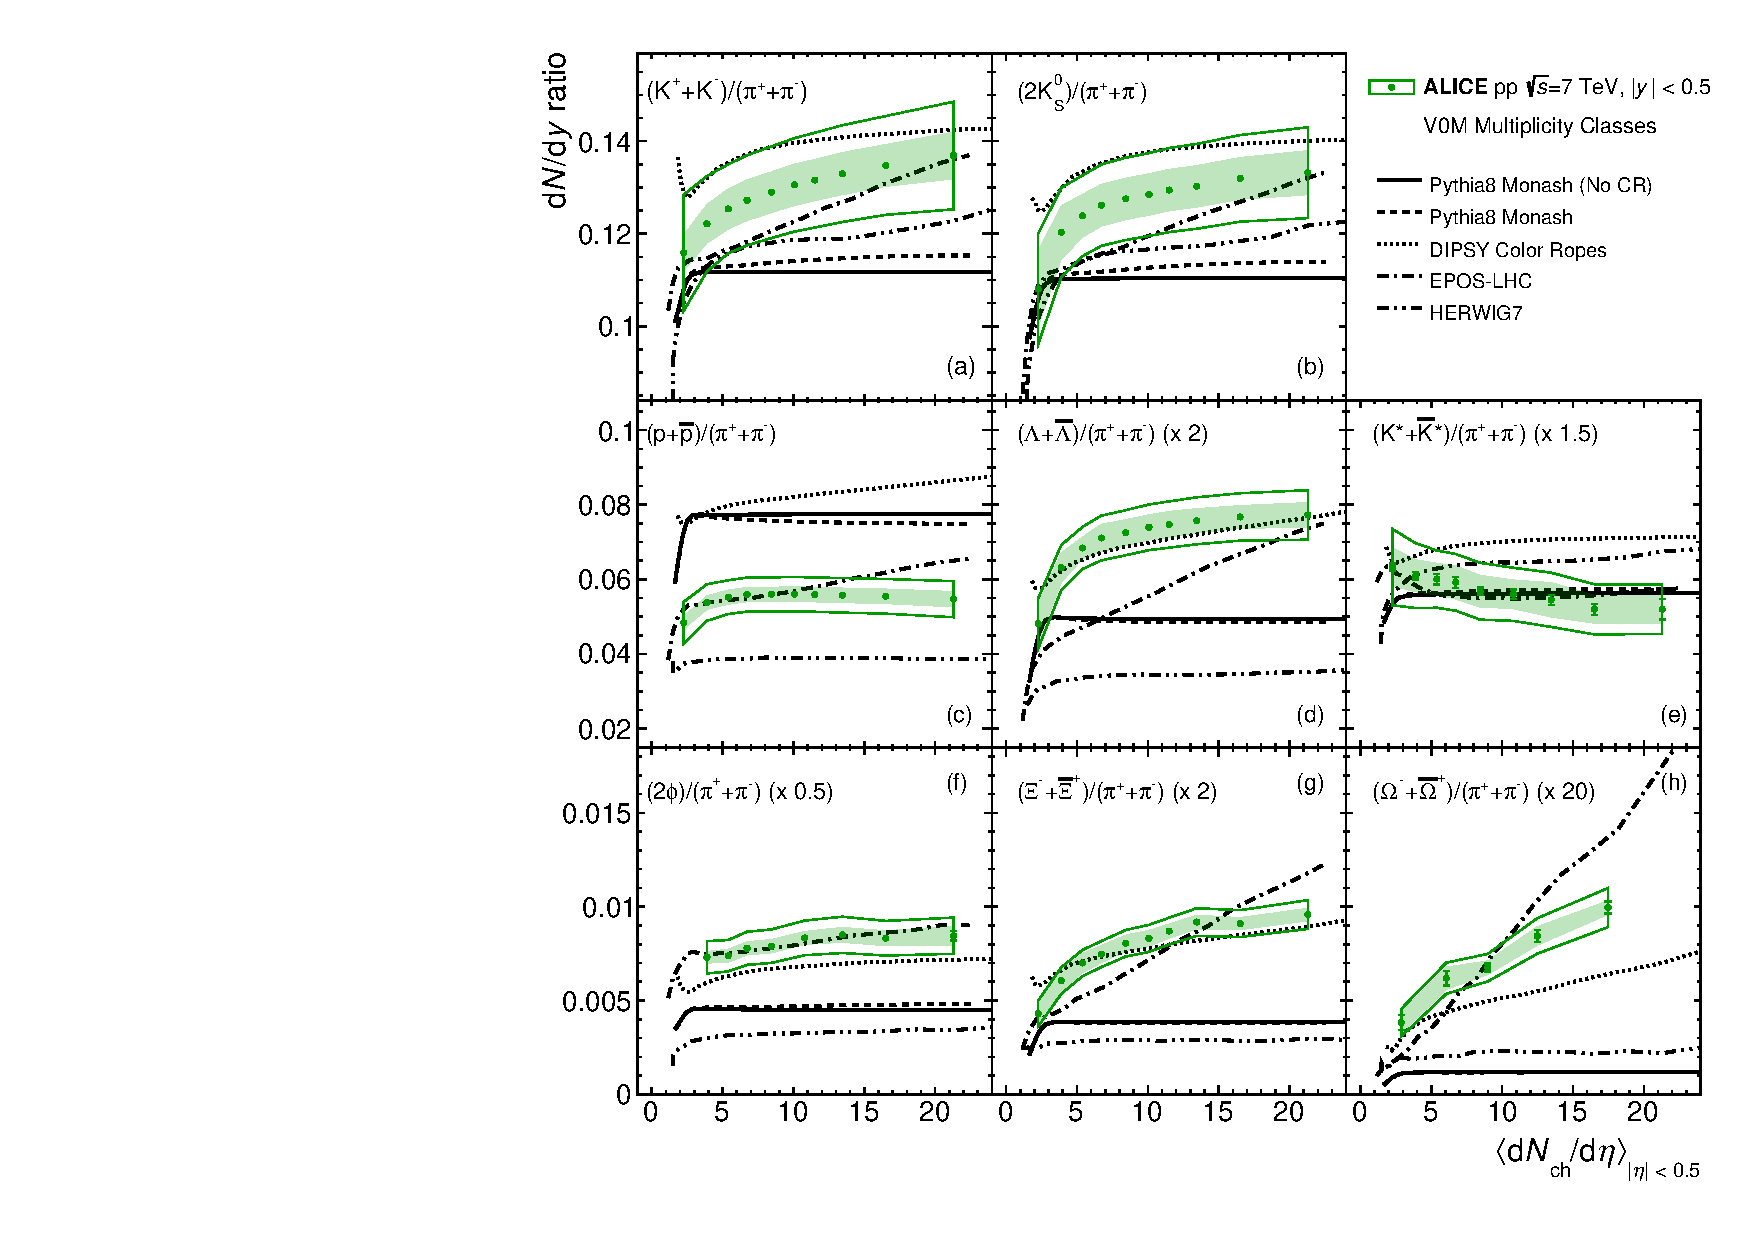
\includegraphics[width=\textwidth]{figures/Discussion_dNdyRatiosVsMC.pdf}} 
    \end{flushleft}
    \caption{Integrated yield ratios as a function of charged-particle multiplicity density compared to several 
Monte Carlo event generators. Statistical uncertainties are shown as error bars, total systematic uncertainties are shown as hollow bands and multiplicity-uncorrelated 
    systematic uncertainties are shown as shaded bands. For a complete description, please refer to the text.} 
    \label{fig:dNdyRatiosVsMC}
\end{figure*}  

The \pt-integrated ratios are compared to predictions from the same Monte Carlo event generators 
in Fig.~\ref{fig:dNdyRatiosVsMC}. The PYTHIA8 and HERWIG generators incorrectly predict no multiplicity dependence of
relative strangeness production and therefore fail especially in the description of multi-strange baryon production, 
while DIPSY and EPOS-LHC exhibit increased strangeness in high-multiplicity 
pp collisions but fail to predict a flat \pTopi\ ratio. None of the tested generators correctly reproduces
the multiplicity dependence of the \kstar/\pion\ ratio, which is observed to decrease slightly. This comprehensive set of measurements provides essential input for all models aiming to describe flavor generation in \pp\ collisions. 

